\documentclass[a4paper,12pt]{article}

\usepackage{cmap}					
\usepackage[T2A]{fontenc}			
\usepackage[utf8]{inputenc}			
\usepackage[english,russian]{babel}	

\usepackage{amsmath,amsfonts,amssymb,amsthm,mathtools} 
\usepackage{wasysym}


\usepackage{graphicx}
\usepackage[cache=false]{minted}

\usepackage{indentfirst}
\usepackage{amssymb}


\usepackage{listings} 
\usepackage{fancyvrb}
%\DefineShortVerb{\|}

\usepackage{color}
\usepackage{caption}
\DeclareCaptionFont{white}{\color{black}}
\DeclareCaptionFormat{listing}{\colorbox{white}{\parbox{\textwidth}{#1#2#3}}}
\captionsetup[lstlisting]{format=listing,labelfont=white,textfont=white}


\usepackage{listings}

\usepackage{geometry}
\geometry{left=2cm}
\geometry{right=1.5cm}
\geometry{top=1cm}
\geometry{bottom=2cm}
\setlength{\parindent}{5ex}
\setlength{\parskip}{0.5em}

\begin{document} % Конец преамбулы, начало текста.

\lstset{ %
language=C++,                 % выбор языка для подсветки (здесь это С)
basicstyle=\small\sffamily, % размер и начертание шрифта для подсветки кода
numbers=left,               % где поставить нумерацию строк (слева\справа)
numberstyle=\tiny,           % размер шрифта для номеров строк
stepnumber=1,                   % размер шага между двумя номерами строк
numbersep=5pt,                % как далеко отстоят номера строк от подсвечиваемого кода
backgroundcolor=\color{white}, % цвет фона подсветки - используем \usepackage{color}
showspaces=false,            % показывать или нет пробелы специальными отступами
showstringspaces=false,      % показывать или нет пробелы в строках
showtabs=false,             % показывать или нет табуляцию в строках
frame=single,              % рисовать рамку вокруг кода
tabsize=2,                 % размер табуляции по умолчанию равен 2 пробелам
captionpos=t,              % позиция заголовка вверху [t] или внизу [b] 
breaklines=true,           % автоматически переносить строки (да\нет)
breakatwhitespace=false, % переносить строки только если есть пробел
escapeinside={\%*}{*)}   % если нужно добавить комментарии в коде
}

\large
\begin{center}
Федеральное государственное бюджетное образовательное учреждение высшего образования «Московский государственный технический университет имени Н. Э. Баумана (национальный исследовательский университет»)
\end{center}

\vspace*{30mm} 

\LARGE
\begin{center}
Курс: <<Анализ алгоритмов>>

Лабораторная работа №1
\end{center}

\vspace*{30mm} 

\huge
\begin{center}
Тема работы:\\
<<Расстояние Левенштейна и Дамерау-Левенштейна>>
\end{center}
\vspace*{30mm} 

\large
\begin{flushright}
Студент: Волков Е. А. \\
Преподаватели: Волкова Л. Л. \\
				Строганов Ю. В. \\
Группа: ИУ7-55Б
\end{flushright}

\vspace*{40mm}
\begin{center}
2019    
\end{center}

\thispagestyle{empty}
\pagebreak

\tableofcontents
\pagebreak


\section*{Введение}
\addcontentsline{toc}{section}{Введение}

При создании программного продукта может возникнуть необходимость сравнить текстовый запрос пользователя с некоторой базой слов и если совпадение не будет найдено, найти ближайшие к написанному слова. 

Цель лабораторной работы: изучение метода динамического программирования на материале алгоритмов
Левенштейна и Дамерау-Левенштейна.

Задачи работы:

\begin{enumerate} 
	\item[1)] изучение алгоритмов Левенштейна и Дамерау-Левенштейна нахождения 
	расстояния между
	строками;
	\item[2)] применение метода динамического программирования для матричной 
	реализации указанных
	алгоритмов;
	\item[3)] получение практических навыков реализации указанных алгоритмов: двух
	алгоритмов в
	матричной версии и одного из алгоритмов в рекурсивной версии;
	\item[4)] сравнительный анализ линейной и рекурсивной реализаций выбранного
	алгоритма
	определения расстояния между строками по затрачиваемым ресурсам (времени и
	памяти);
	\item[5)] экспериментальное подтверждение различий во временнóй эффективности
	рекурсивной и
	нерекурсивной реализаций выбранного алгоритма определения расстояния между
	строками при
	помощи разработанного программного обеспечения на материале замеров
	процессорного времени
	выполнения реализации на варьирующихся длинах строк;
	\item[6)] описание и обоснование полученных результатов в отчете о выполненной
	лабораторной
	работе, выполненного как расчётно-пояснительная записка к работе. 
\end{enumerate} 
\pagebreak



\section{Аналитический раздел}
	
	В данном разделе анализируются наиболее популярные алгоритмы для нахождения расстояний Левенштейна и Дамерау-Левенштейна. 
	
 
	
	\subsection{Описание алгоритмов}
		Определим редакторские операции над строкой s:
		    \begin{enumerate} 
		        \item I - вставка (insert) - цена 1;
		        \item D - удаление (delete) - цена 1;
		        \item R - замена (replace) - цена 1;
		        \item M - совпадение (match) - цена 0.
		    \end{enumerate} 
		    
		Расстояние Левенштейна  — это минимальное количество операций вставки одного символа, удаления одного символа и замены одного символа на 
другой, необходимых для превращения одной строки в другую.
		     
		Этот алгоритм активно применяется в следующих областях:
	\begin{enumerate}
	\item[1)]для исправления ошибок в слове (в поисковых системах, базах данных, при вводе текста, при автоматическом распознавании отсканированого текста или речи);
	\item[2)]для сравнения текстовых файлов утилитой diff и ей подобными. Здесь роль «символов» играют строки, а роль «строк» — файлы;
	\item[3)]в биоинформатике для сравнения генов, хромосом и белков~\cite{primenenie}.
	\end{enumerate}
	
	    \subsubsection{Расстояние Левенштейна}
	   
		    
		     Пусть $S_{1}$ и $S_{2}$ — две строки (длиной M и N соответственно) над 
		     некоторым алфавитом, тогда расстояние Левенштейна $d(S_{1}, S_{2})$ 
		     можно подсчитать по следующей рекуррентной формуле $d(S_{1}, S_{2}) = 
		     D(M, N)$, где:	    
		    
		    \begin{equation}
		     D(i, j) =  \left\{
			\begin{aligned}
				&0, && i = 0, j = 0\\
		    	&i, && i > 0, j = 0\\
		    	&j, && i = 0, j > 0\\
		    	&min \left\{
				\begin{aligned}
					&D(i, j - 1) + 1,\\
		            &D(i - 1, j) + 1, \\
		            &D(i - 1, j - 1) + m(S_{1}[i], S_{2}[j]),\\
		        \end{aligned} \right. &&i > 0, j > 0,
			\end{aligned} \right.
			\label{eq_lev}
			\end{equation}
				    
		    где $m(S_{1}[i], S_{2}[i])$  равна нулю, если $S_{1}[i] = S_{2}[j]$ и 					единице в противном случае. ~\cite{lev_pas} \\
		     		
		    
	  	\subsubsection{Расстояние Дамерау-Левенштейна}
		    Расстояние Дамерау - Левенштейна является модификацией расстояния Левенштейна. Оно получается, если к списку разрешённых операций добавить транспозицию (два соседних символа меняются местами). Цена транспозиции, также как и для вставки, удаления и замены, равняется 1~\cite{dam_lev_habr}.
	
		    
		    Пусть, как в формуле \ref{eq_lev}, $S_{1}$ и $S_{2}$ — две строки (длиной M и N соответственно) над некоторым алфавитом, тогда расстояние Левенштейна $d(S_{1}, S_{2})$ можно подсчитать по следующей рекуррентной формуле $d(S_{1}, S_{2}) = D(M, N)$, где:
		    
		     \[ D(i, j) =  \left\{
			\begin{aligned}
				&0, && i = 0, j = 0\\
		    	&i, && i > 0, j = 0\\
		    	&j, && i = 0, j > 0\\		    	
		    	&min \left\{
				\begin{aligned}
					&D(i, j - 1) + 1,\\
		            &D(i - 1, j) + 1,\\
		            &D(i - 1, j - 1) + m(S_{1}[i], S_{2}[i]), \\
		            &D(i - 2, j - 2) + m(S_{1}[i], S_{2}[i]),\\
		        \end{aligned} \right.
		        && 
				\begin{aligned}
					&, \text{ если } i, j > 0 \\
		            & \text{ и } S_{1}[i] = S_{2}[j - 1] \\
		            & \text{ и } S_{1}[i - 1] =  S_{2}[j] \\
		        \end{aligned} \\ 
		        &min \left\{
		        \begin{aligned}
		            &D(i, j - 1) + 1,\\
		            &D(i - 1, j) + 1, \\
		            &D(i - 1, j - 1) + m(S_{1}[i], S_{2}[i]),\\
		        \end{aligned} \right.  &&, \text{иначе}.
			\end{aligned} \right.
			\]	
	    
		\subsection*{Вывод}
		\addcontentsline{toc}{subsection}{Вывод}
		В данном разделе были рассмотрены алгоритмы нахождения расстояния Левенштейна и Дамерау-Левенштейна, который является модификаций первого, учитывающего возможность перестановки соседних символов. 


\pagebreak


\section{Конструкторский раздел}
	В данном разделе содержатся схемы алгоритмов.
	
%	 и сравнение матричного и рекурсивного способов нахождения расстояний Левенштейна и Дамерау-Левенштейна
       
    
        
        
    \subsection{Разработка алгоритмов}
    
        На рис. \ref{fig:schema_lev_matr} приведена схема матричного алгоритма 					Левенштейна.
        
        \begin{figure}[h!]
        	\begin{center}
        		{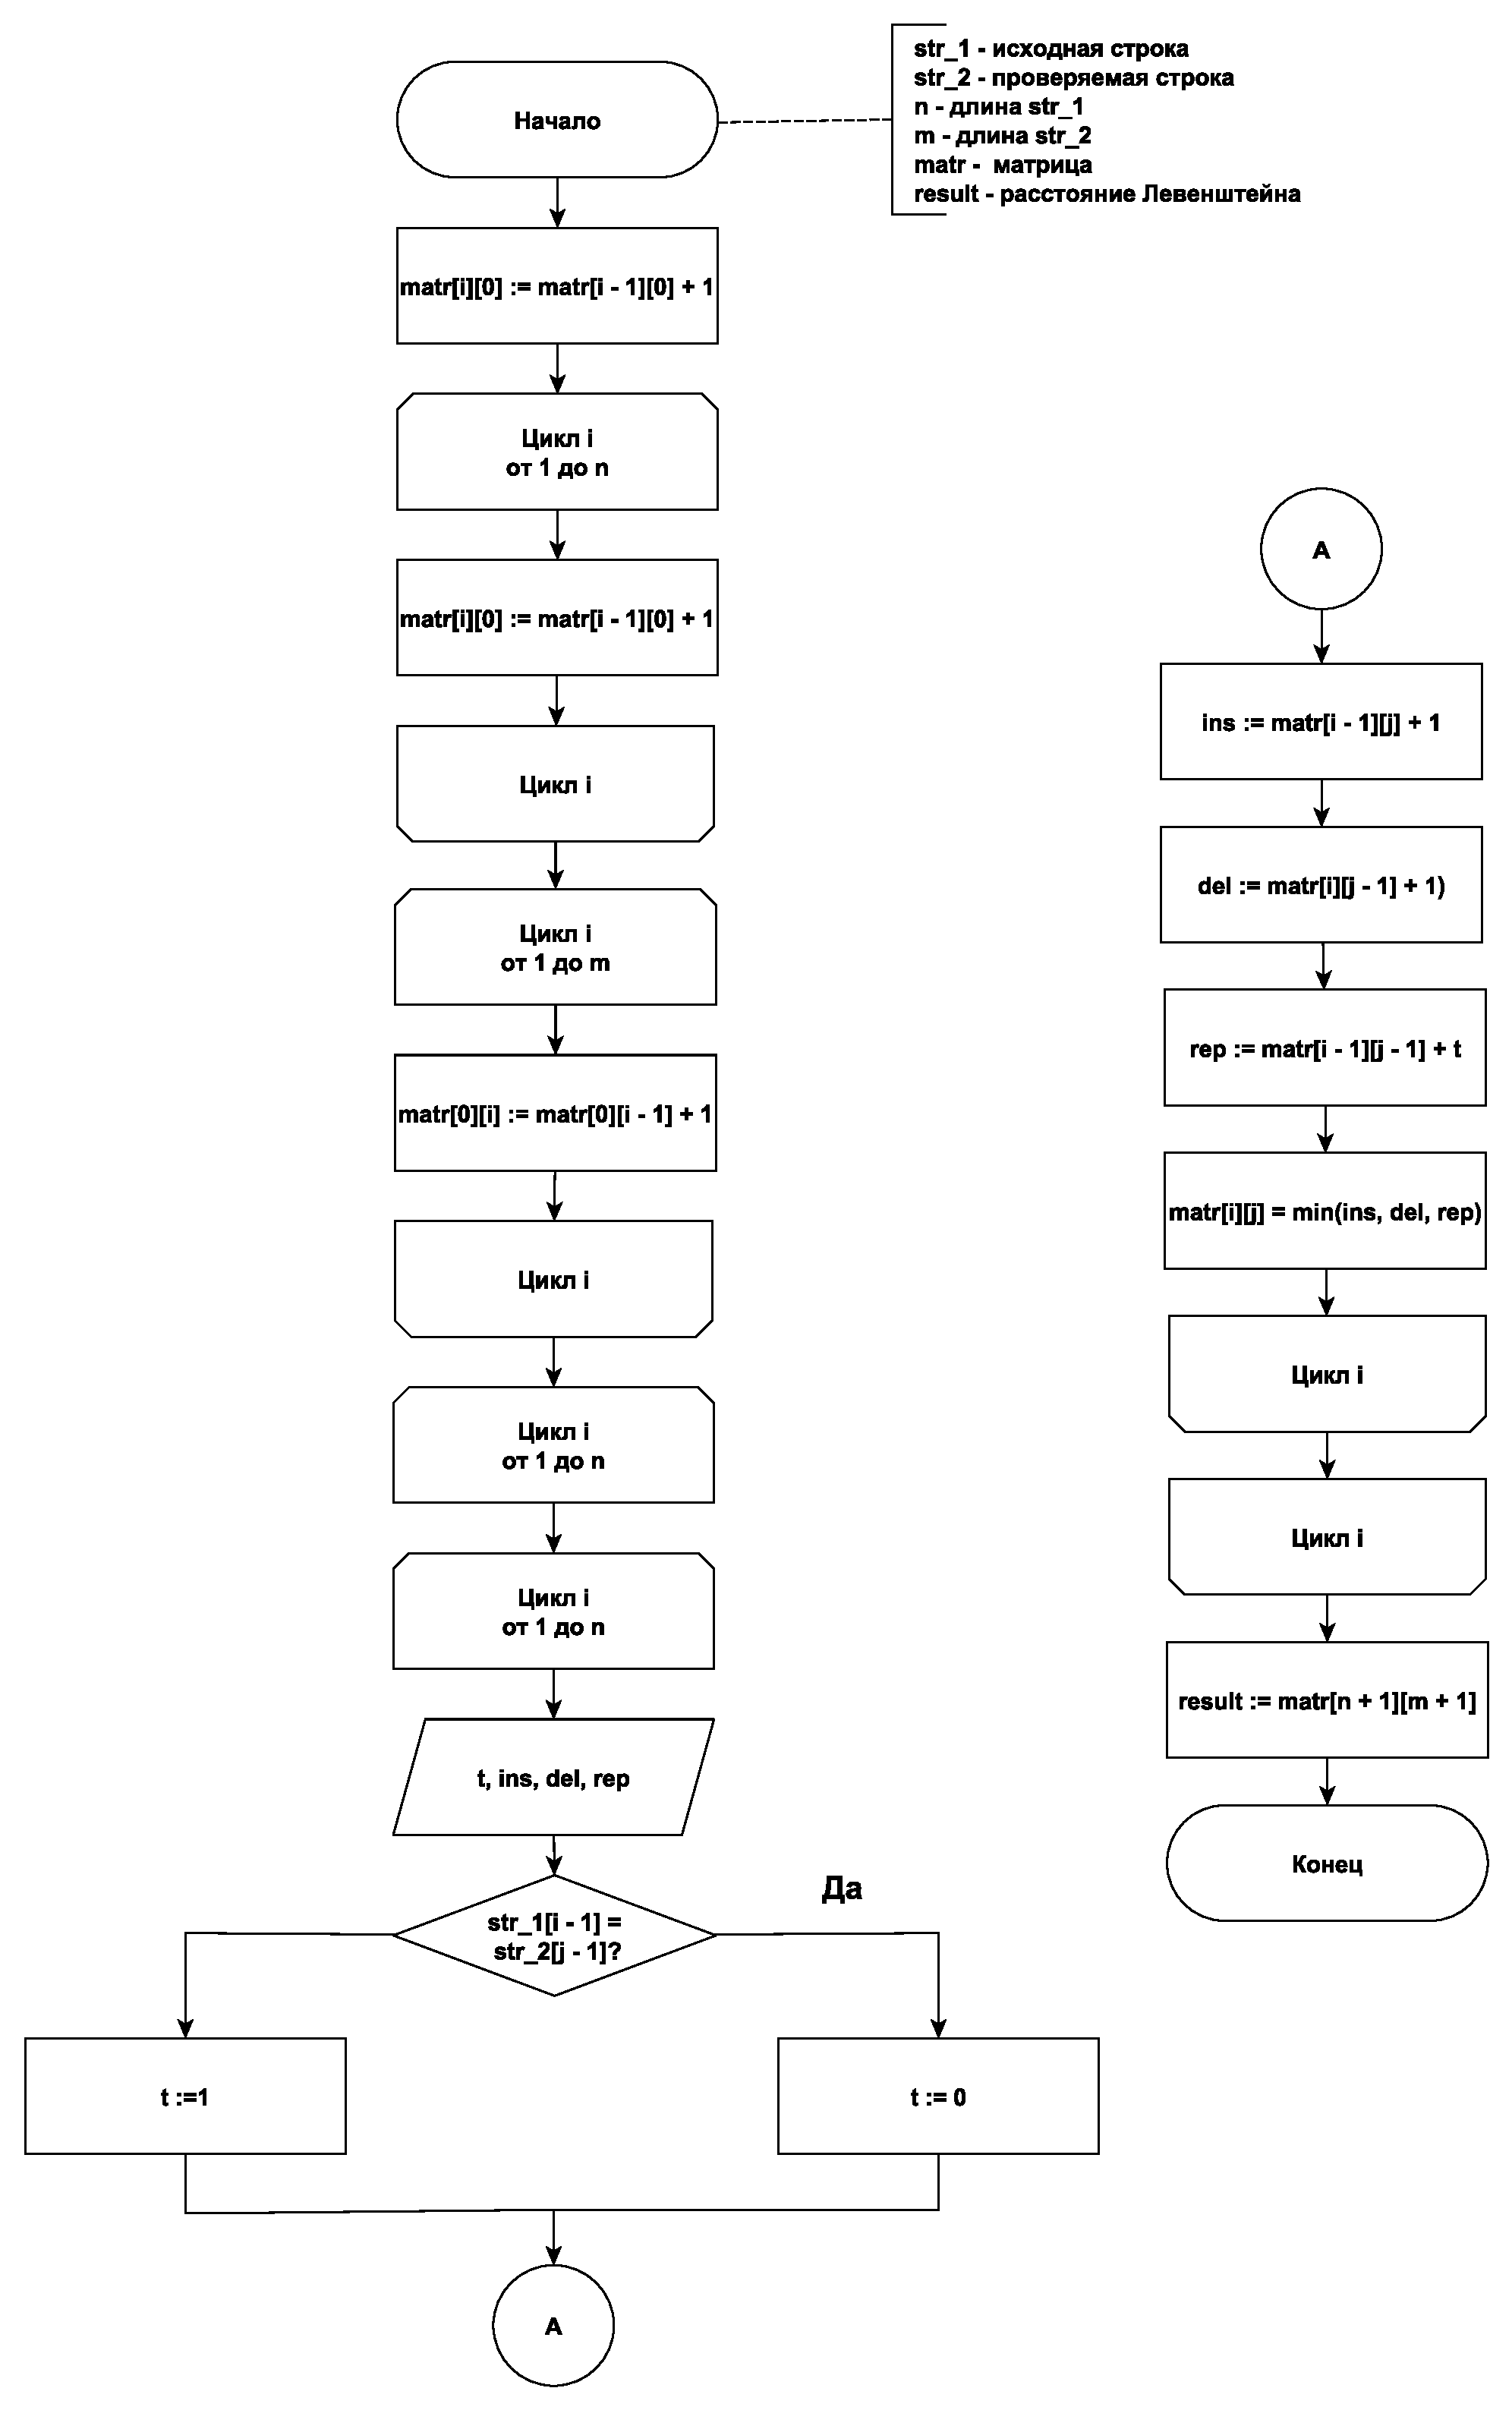
\includegraphics[scale = 0.37]{schema02.pdf}}
        		\caption{Матричный алгоритм нахождения расстояния Левенштейна}
        		\label{fig:schema_lev_matr}
        	\end{center}
        \end{figure}
        
        На рис. \ref{fig:schema_dam_lev_matr} приведена схема матричного алгоритма 				Левенштейна.
        
        \begin{figure}[h!]
        	\begin{center}
        		{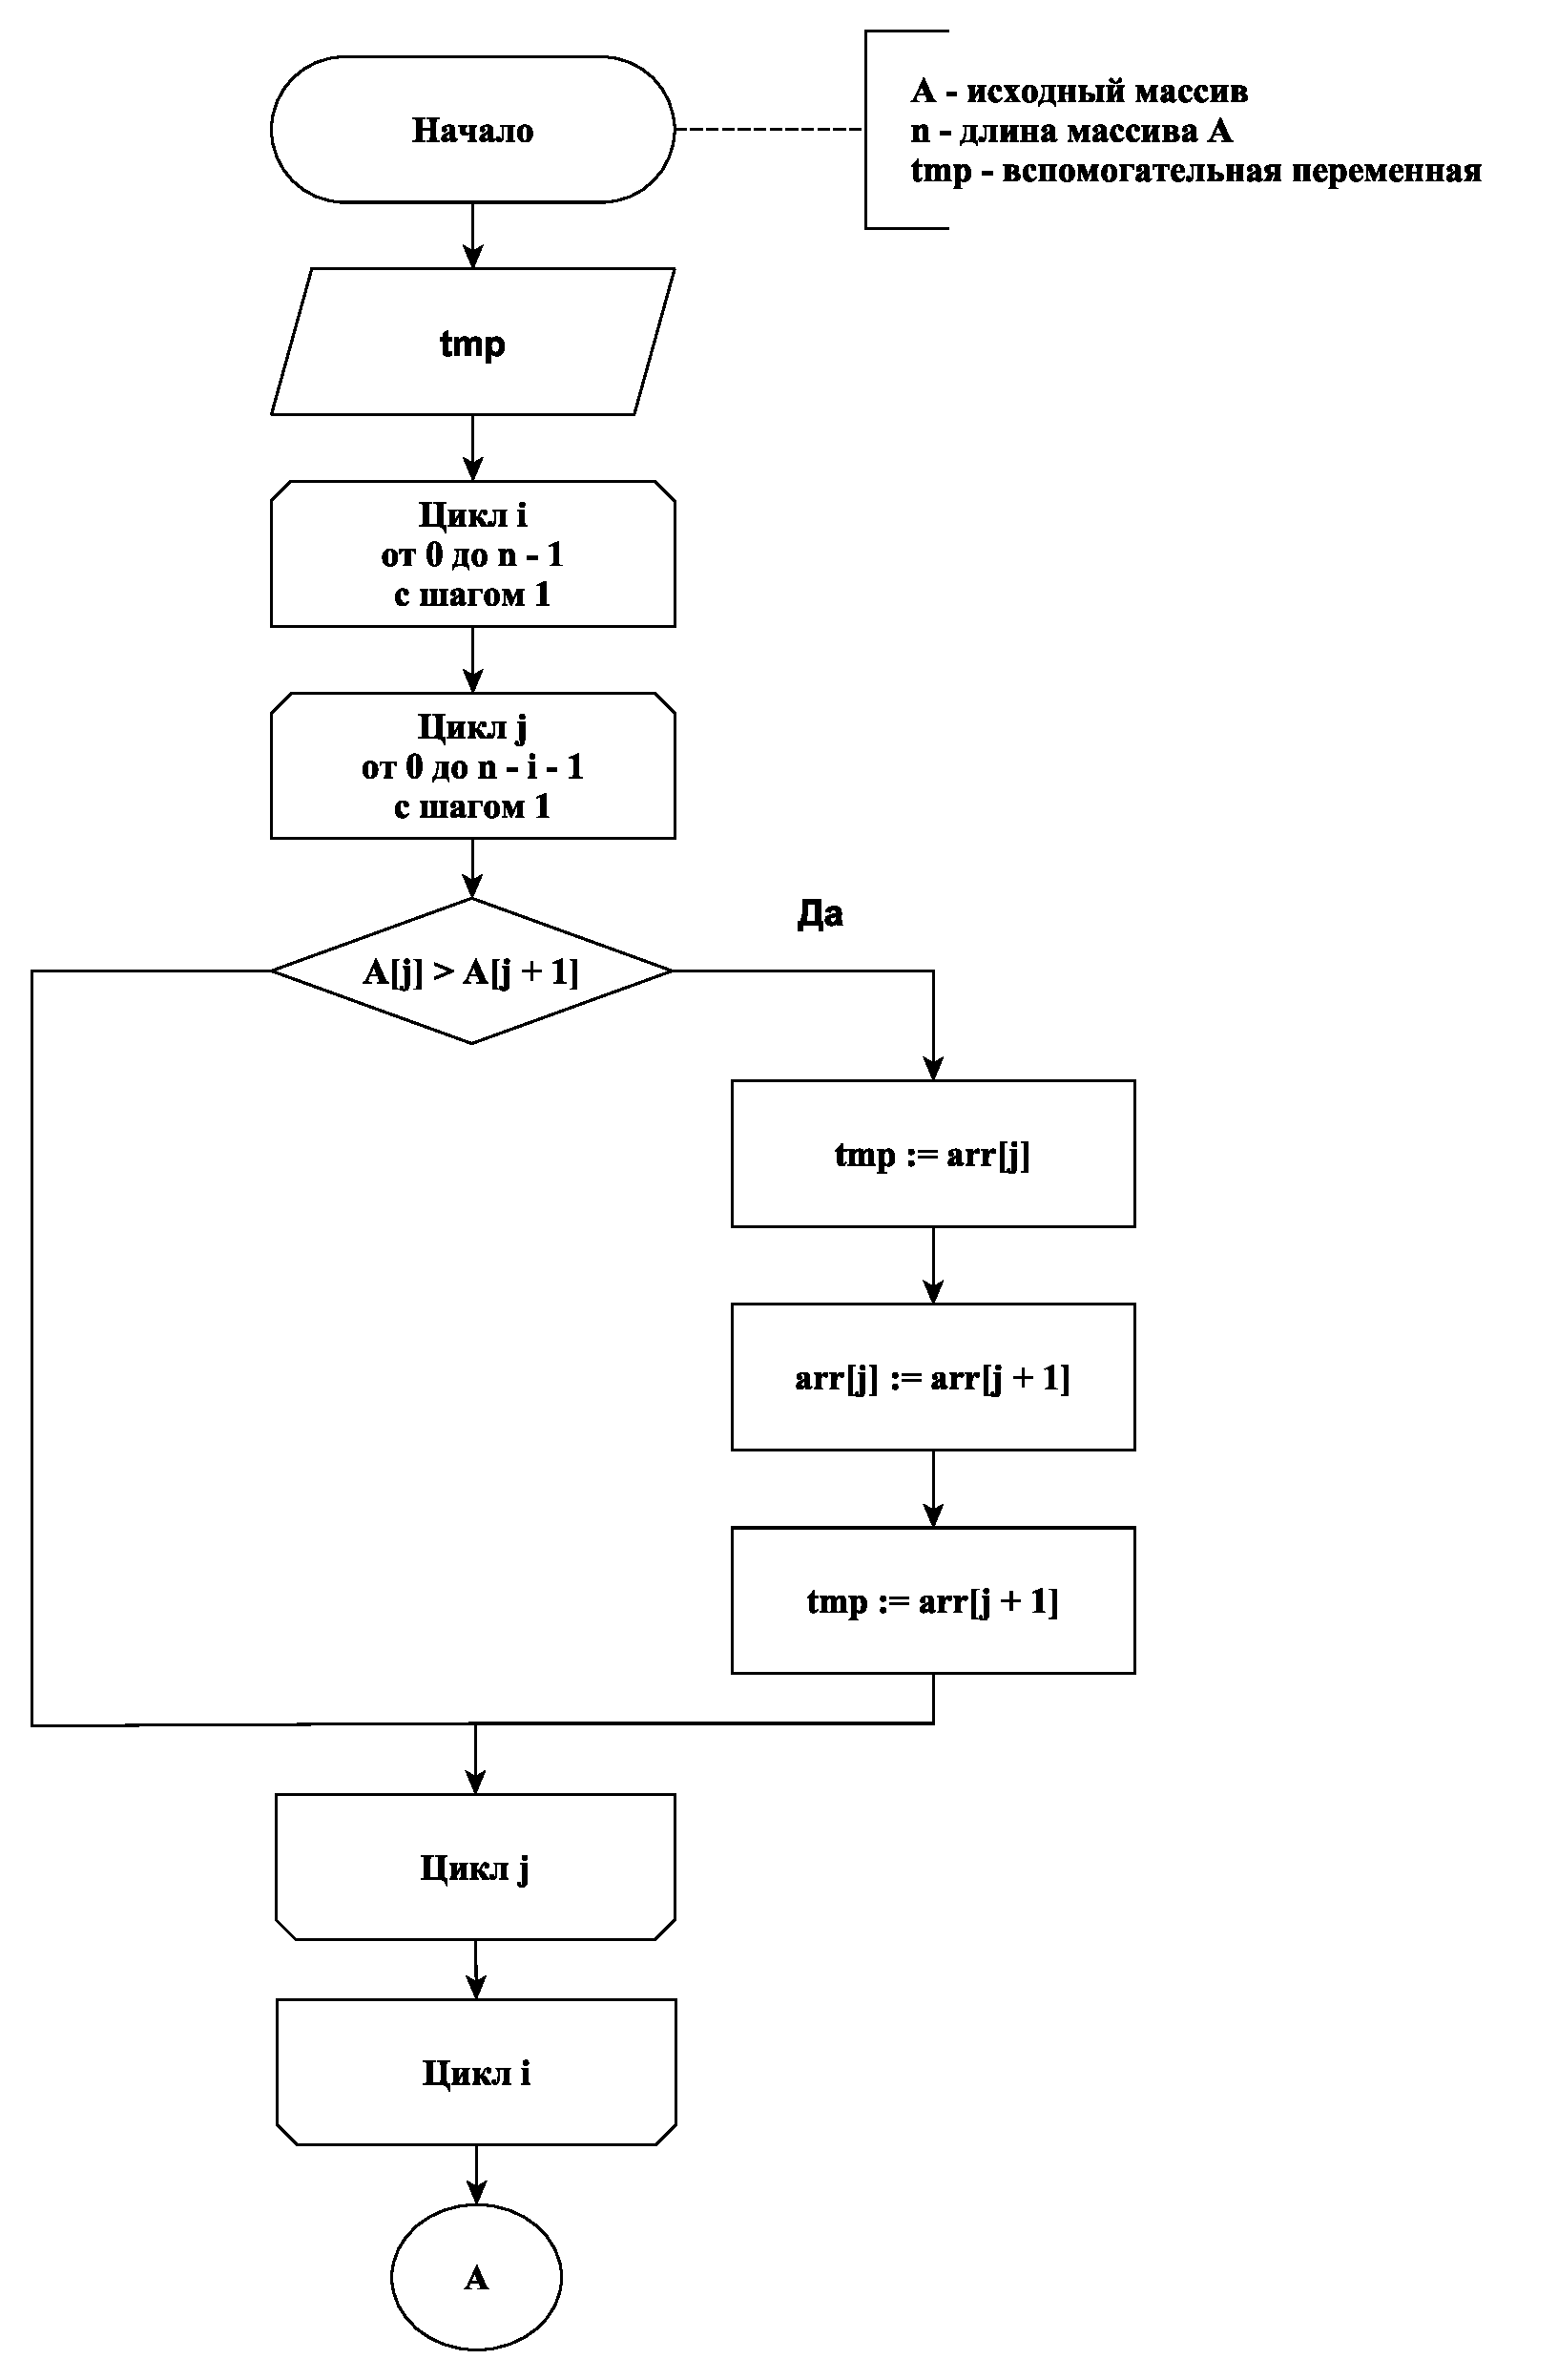
\includegraphics[width = \textwidth]{schema01.pdf}}
        		\caption{Матричный алгоритм нахождения расстояния Дамерау-								Левенштейна}
        		\label{fig:schema_dam_lev_matr}
        	\end{center}
        \end{figure}
    

	    На рис. \ref{fig:schema_dam_lev_rec} приведена схема рекурсивного алгоритма 			Дамерау-Левенштейна.
	    
	    \begin{figure}[h!]
	    	\begin{center}
	    		{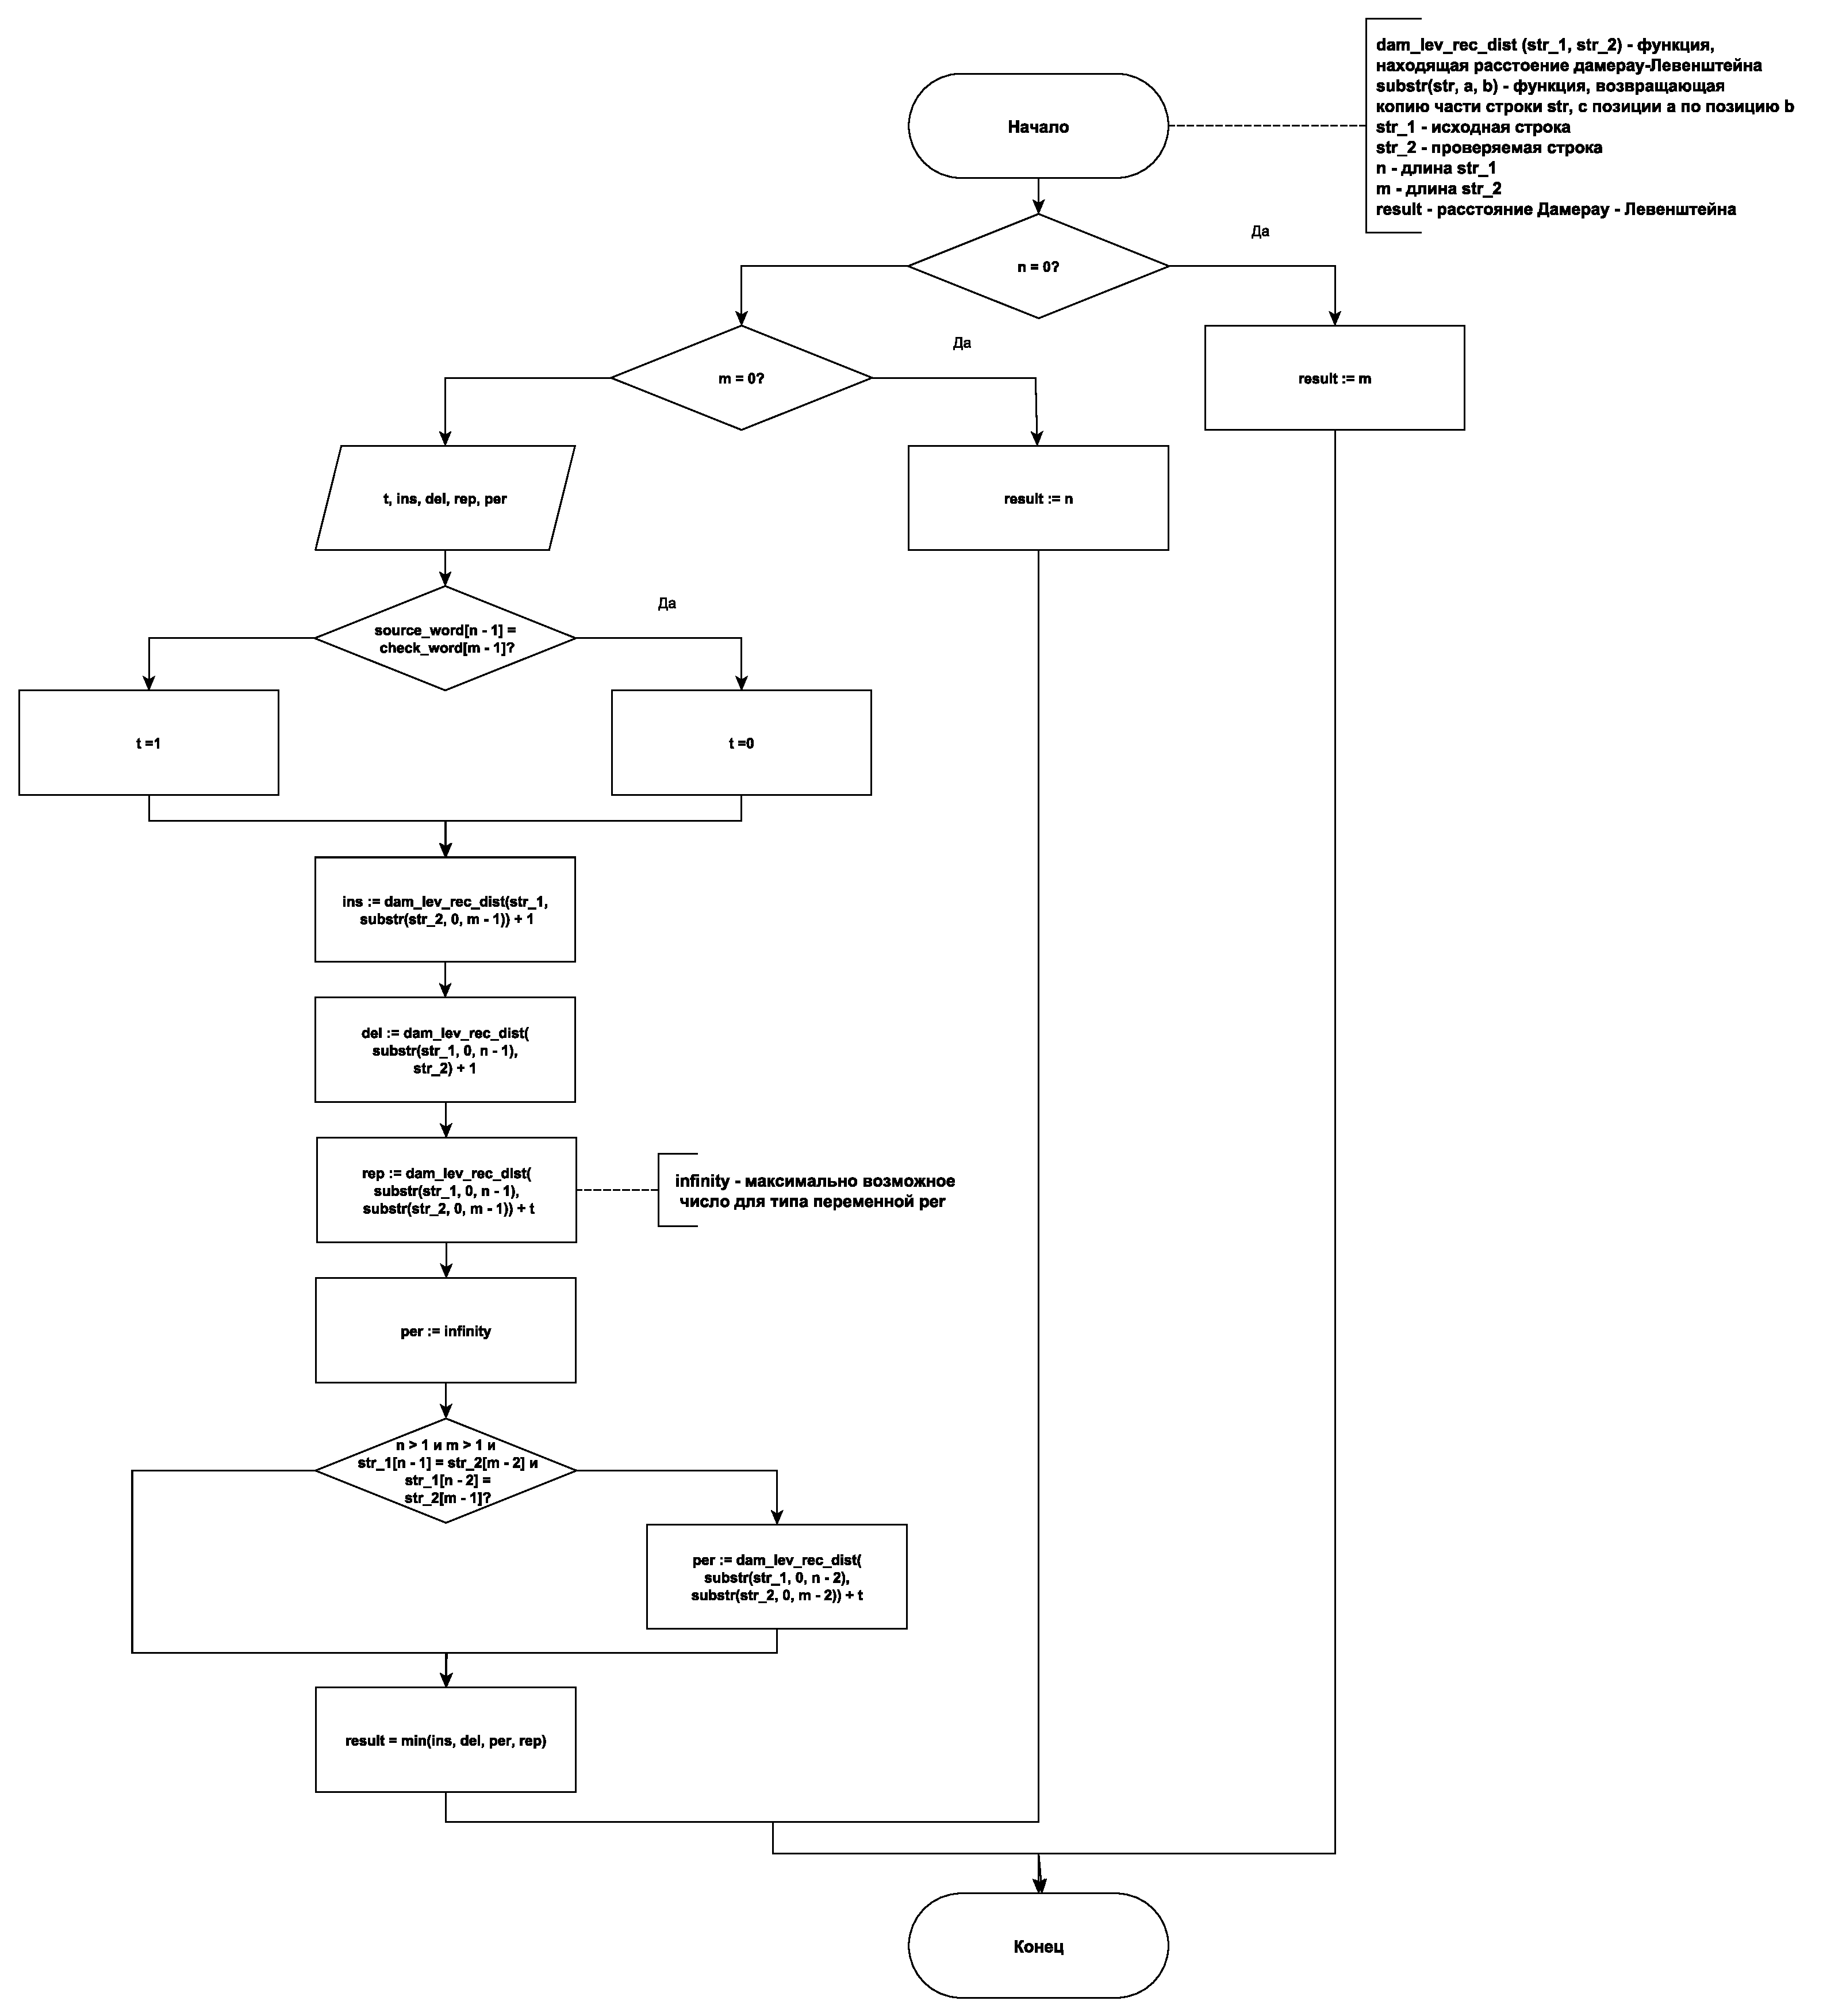
\includegraphics[width = \textwidth]{schema03.pdf}}
	    		\caption{Рекурсивный алгоритм нахождения расстояния Дамерау-							Левенштейна}
	    		\label{fig:schema_dam_lev_rec}
	    	\end{center}
	    \end{figure}
	    
	\subsection*{Вывод}
		\addcontentsline{toc}{subsection}{Вывод}
	В данном разделе были представлены схемы матричного алгоритма Левенштейна и 				матричного и рекурсивного алгоритмов Дамерау-Левенштейна.


	
	 
	
    
\pagebreak    

\section{Технологический раздел}

	В данном разделе будут описаны требования к программному обеспечению и средства реализации, приведён листинг программ и проведен сравнительный анализ потребления алгоритмами памяти.
	\subsection{Требования к программному обеспечению}
	Входные данные: две строки (возможно пустые) с любыми символами.
	
	Выходные данные: численное значение расстояний Левенштейна и Дамерау - Левенштейна
	
	На рис. \ref{fig:idef0} приведена функциональная схема определения расстояния Девенштейна (Дамерау - Левенштейна).
        
        \begin{figure}[h!]
        	\begin{center}
        		{\includegraphics[width = \textwidth]{idef0.png}}
        		\caption{Функциональная схема определения расстояния Левенштейна (Дамерау - Левенштейна)}
        		\label{fig:idef0}
        	\end{center}
        \end{figure}
        
	
	\subsection{Средства реализации}
	Программа написана на языке С++, т. к. этот язык предоставляет программисту широкие возможности реализации самых разнообразных алгоритмов, обладает высокой эффективностью и значительным набором стандартных классов и процедур. В качестве среды разработки использовался  фреймворк QT 5.13.1.
	
	Для обработки строк и матриц были использованы стандартные контейнерные классы std::string и std::vector.
	
	Для замера времени выполнения программы использовалась библиотека ctime.
	

    
    \subsection{Листинг программы}
	
	В листингах \ref{code_lev},  \ref{code_dam_lev_m} и \ref{code_dam_lev_r} представлены функции, описывающие матричную реализацию алгоритма Левенштейна и матричную и рекурсивную реализацию алгоритма Дамерау - Левенштейна
	\begin{center}
	\begin{lstlisting}[label=code_lev, caption={Матричный алгоритм Левенштейна}]

int lev_matr_dist(string source_word, string check_word) {
    size_t n = source_word.size() + 1;
    size_t m = check_word.size() + 1;
    Matrix matr(n, Vector(m, 0));

    for(size_t i = 1; i < n; i++) {
        matr[i][0] = matr[i - 1][0] + 1;
    }

    for(size_t i = 1; i < m; i++) {
        matr[0][i] = matr[0][i - 1] + 1;
    }

    for (size_t i = 1; i < n; i++) {
        for(size_t j = 1; j < m; j++) {
            source_word[i - 1] == check_word[j - 1] ? t = 0 : t = 1;
            matr[i][j] = min(min(matr[i - 1][j] + 1, matr[i][j - 1] + 1),
                    matr[i - 1][j - 1] + t);
        }
    }

    //print_matr(matr, source_word, check_word);
    return matr[n - 1][m - 1];
}
	\end{lstlisting}  
	\end{center}
    
\begin{lstlisting}[label=code_dam_lev_m, caption={Матричный алгоритм Дамерау - Левенштейна}]     

int dam_lev_matr_dist(string source_word, string check_word) {
    size_t n = source_word.size() + 1;
    size_t m = check_word.size() + 1;
    Matrix matr(n, Vector(m, 0));

    for(size_t i = 1; i < n; i++) {
        matr[i][0] = matr[i - 1][0] + 1;
    }

    for(size_t i = 1; i < m; i++) {
        matr[0][i] = matr[0][i - 1] + 1;
    }

    for (size_t i = 1; i < n; i++) {
        for(size_t j = 1; j < m; j++) {
            t = 0;
            source_word[i - 1] == check_word[j - 1] ? t = 0 : t = 1;
            matr[i][j] = min(min(matr[i - 1][j] + 1, matr[i][j - 1] + 1),
                    matr[i - 1][j - 1] + t);

            if (i > 1 && j > 1 && source_word[i - 1] == check_word[j - 2] &&
                    source_word[i - 2] == check_word[j - 1]) {
                matr[i][j] = min(matr[i][j], matr[i - 2][j - 2] + t);
            }
        }
    }

    print_matr(matr, source_word, check_word);
    return matr[n - 1][m - 1];
}
\end{lstlisting}

\begin{lstlisting}[label=code_dam_lev_r, caption={Матричный алгоритм Дамерау - Левенштейна}]     

int dam_lev_rec_dist(string source_word, string check_word) {

    size_t n = source_word.size();
    size_t m = check_word.size();

    if (!n) {
        return m;
    }
    if (!m) {
        return n;
    }

    int t = 0;
    source_word[n - 1] == check_word[m - 1] ? t = 0 : t = 1;

    int ins = dam_lev_rec_dist(source_word, check_word.substr(0, m - 1)) + 1;
    int del = dam_lev_rec_dist(source_word.substr(0, n - 1), check_word) + 1;
    int rep = dam_lev_rec_dist(source_word.substr(0, n - 1), 
                               check_word.substr(0, m - 1)) + t;
    int per = std::numeric_limits<short>::max();

    if (n > 1 && m > 1 && source_word[n - 1] == check_word[m - 2] &&
            source_word[n - 2] == check_word[m - 1]) {
        per = dam_lev_rec_dist(source_word.substr(0, n - 2),
                                         check_word.substr(0, m - 2)) + t;
    }
    
    return min(min(min(ins, del), rep), per);
}

\end{lstlisting}  
    
%    
    \subsection{Тестовые данные}
    \label{fig:test_data}

    Программа должна корректно находить расстояния Левенштейна и Дамерау-Левенштейна при следующих входных данных, представленных в таблице \ref{table:test_data_table}.\\
    \begin{table} [h!]
    \begin{center}
    \caption{Тестовые данные} 
    \begin{tabular}{|c|p{3.5cm}|p{3.5cm}|p{3.5cm}|p{3.5cm}|}
    	\hline
    	№ & Исходное слово & Проверяемое слово & Расстояние Левенштейна & Расстояние Дамерау - Левенштейна\\
    	\hline
    	1 & \diameter & \diameter & 0 & 0  \\
    	\hline
    	2 & \diameter & a & 1 & 1  \\
    	\hline
    	3 & a & \diameter & 1 & 1  \\
    	\hline
    	4 & a & a & 1 & 1  \\
    	\hline
    	5 & skat & kot & 2 & 2  \\
    	\hline
    	6 & red & erd & 2 & 1  \\
    	\hline
    	7 & student & sutednt & 3 & 2  \\
    	\hline
    	8 & mouse & mouse & 0 & 0  \\
    	\hline
    	9 & elephant & relevant & 3 & 3  \\
    	\hline
    	10 & abc & def & 3 & 3  \\
    	\hline
    	11 & coffee & soda & 1 & 1  \\
    	\hline
    	12 & annas & max & 4 & 4  \\
    	\hline
    	13 & levenshtein & meilenstein & 4 & 4  \\
    	\hline
    	14 & notebook & ontbeooko & 5 & 3  \\
    	\hline
    	15 & market & street & 3 & 3  \\
    	\hline
    	16 & ball & ballon & 2 & 2  \\
    	\hline
    	17 & bbball & ball & 2 & 2  \\
    	\hline
    	18 & doctor & odtcor & 3 & 2  \\
    	\hline
    	19 & factory & fcatroy & 4 & 2  \\
    	\hline
    	20 & park & krap & 4 & 3  \\
    	\hline
    \end{tabular} \\

    \label{table:test_data_table}
    \end{center}
    \end{table}
    
    Расстояние Дамерау-Левенштейна, посчитанное рекурсией и расстояние Дамерау-Левенштейна, посчитанное с помощью матрицы должны совпадать.

	\subsection{Сравнительный анализ рекурсивной и нерекурсивной реализаций}
	
	Расчёт потребляемой памяти для матричного алгоритма Дамерау-Левенштейна для двуx строк размерами n и m приведен в таблице \ref{table:table_memory_1}:
	\begin{table} [h!]
	\begin{center}
	\caption{Расчёт используемой памяти для матричного алгоритма Дамерау-Левенштейна}
	\begin{tabular}{|p{4cm}|p{6cm}|p{5cm}|}
	\hline 
	Объект & Занимаемая память (формула)  & Занимаемая память (байт) \\ 
	\hline 
	Матрица & sizeof(std::vector) & 24 \\ 
	\hline 
	Строки матрицы & (n + 1)*sizeof(std::vector) & (n + 1)*24 \\ 
	\hline 
	Ячейки матрицы & (n + 1)*(m + 1)*sizeof(int) & (n + 1)*(m + 1)*4 \\ 
	\hline 
	Вспомогательные переменные  & 3*sizeof(int) & 3*4 \\ 
	\hline 
	\end{tabular} \\
    \label{table:table_memory_1}
    \end{center}
	\end{table}
	
	
	Таким образом, общая формула будет выглядеть так:
	\begin{equation}
	Memory = 24 + (n + 1)*24 + (n + 1)*(m + 1)*4 + 3*4.
	\label{eq:mem_1}
	\end{equation}
	
	
	В алгоритме Левенштейна используется на одну вспомогательную переменную меньше, поэтому формула будет отличаться незначительно:
	
	\[Memory = 24 + (n + 1)*24 + (n + 1)*(m + 1)*4 + 2*4.\]
	
	Следовательно, можно считать потребление памяти матричным алгоритмом Левенштейна приблизительно равным потреблению памяти матричным алгоритмом Дамерау-Левенштейна.
	
	В рекурсивном алгоритме Дамерау-Левенштейна максимальное количество занятой памяти зависит от глубины рекурсии. Если n >= m, то рекурсия будет иметь глубину n. Расчёт памяти для i-го рекурсивного вызова представлен в таблице \ref{table:table_memory_2}.
	
	
	\begin{table} [h!]
	\begin{center}
	\caption{Расчёт используемой памяти для i-го рекурсивного вызова алгоритма Дамерау-Левенштейна}
	\begin{tabular}{|p{4cm}|p{6cm}|p{5cm}|}
	\hline 
	Объект & Занимаемая память (формула)  & Занимаемая память (байт) \\ 
	\hline 
	Две строки & sizeof(std::string)*2 & 32*2 \\ 
	\hline 
	Элементы строк  & (m + n - i)*sizeof(char) & m + n - i \\ 
	\hline 
	Область в стеке для нового рекурсивного вызова & адрес возврата и два указателя на строку & 8 + 8*2 \\ 
	\hline 
	Вспомогательные переменные  & 7*sizeof(int) & 7*4 \\ 
	\hline 
	\end{tabular} \\

    \label{table:table_memory_2}
    \end{center}
	\end{table}
	
	Общая формула будет выглядеть так:
	\begin{equation}
	Memory = \sum_{i=0}^{n + m} (32*2 + m + n - i + 8*3 + 7*4).
	\label{eq:mem_2}
	\end{equation}
	
	Или более просто:
	
	\[ Memory = (32*2 + m + n + 8*3 + 7*4)*(n + m) - \sum_{i=0}^{n + m}i. \]
	


	Оценить количество потребляемой алгоритмами памяти на строках фиксированной длины можно по таблицам \ref{table:table_memory_3} и \ref{table:table_memory_4} (возмем маленькую строку длиной 5 символов, среднюю - длиной 50 символов и большую - длиной 1000 символов).
	
	
	\begin{table} [h!]	
	\begin{center}
	\caption{Расчёт используемой памяти для матричного алгоритма Дамерау-Левенштейна для строк длиной 5, 50 и 1000 символов}
	\begin{tabular}{|p{3cm}|p{4cm}|p{1.2cm}|p{1.5cm}|p{2cm}|}

	\hline 
	Объект & Формула & n = 5, m = 5	& n = 50, m = 50 & n = 1000, m = 1000 \\ 
	\hline 
	Матрица & 24 & 24 & 24 & 24 \\ 
	\hline 
	Строки матрицы & (n + 1)*24 & 144 & 1224 & 24024 \\ 
	\hline 
	Ячейки матрицы & (n + 1)*(m + 1)*4 & 144 & 10404 & 4008004 \\ 
	\hline 
	Вспомога-тельные переменные & 3*4 & 12 & 12 & 12 \\ 
	\hline 
	Итого (байт) & 24 + (n + 1)*24 + (n + 1)*(m + 1)*4 + 3*4 & 324 & 11664 & 4032064 \\ 

	\hline 
	\end{tabular} \\
    \label{table:table_memory_3}
    \end{center}
	\end{table}
	
	\begin{table} [h!]	
	\begin{center}
	\caption{Расчёт используемой памяти для рекурсивного алгоритма Дамерау-Левенштейна для строк длиной 5, 50 и 1000 символов}
	\begin{tabular}{|p{3cm}|p{4cm}|p{1.2cm}|p{1.5cm}|p{2cm}|}

	\hline 
	Объект & Формула & n = 5, m = 5	& n = 50, m = 50 & n = 1000, m = 1000 \\ 
	\hline 
	Две строки & 32*2*(n + m) & 640 & 6400 & 128000\\ 
	\hline 
	Элементы строк  & $(m + n)*(m + n) -  \sum_{i=0}^{n + m}i$ & 55 & 4950 & 1999000\\ 
	\hline 
	Область в стеке для нового рекурсивного вызова & 8*3*(n + m) & 240 & 2400 & 48000 \\ 
	\hline 
	Вспомога- тельные переменные  & 7*4*(n + m)  & 280 & 2800 & 56000\\ 
	\hline 
	Итого (байт) & $(32*2 + m + n + 8*3 + 7*4*(m+n) - \sum_{i=0}^{n}i$ & 1215 & 16550 & 2231000 \\ 

	\hline 
	\end{tabular} \\
    \label{table:table_memory_4}
    \end{center}
	\end{table}
	
	Таким образом рекурсивный алгоритм выигрывает по памяти в сравнении
с итеративными алгоритмами при обработке строк большой длины.
	
	
	\subsection*{Вывод}
		\addcontentsline{toc}{subsection}{Вывод}
	
	В данном разделе были рассмотрены требования к программному обеспечению, в качестве средств реализации выбраны язык С++ и фреймворк QT версии 5.13.1, приведён листинг программы и тестовые данные. Было проанализировано потребление каждым из алгоритмов памяти, были выведены формулы для вычисления памяти на строках определенной длины. Аналитическое сравнение потребления памяти алгоритмами на строках длины 5, 50 и 1000 символов показало, что  матричный алгоритм Дамерау-Левенштейна эффективен на строках длиной 5 и 50 символов, а рекурсивный  - на строках длиной 1000 символов.
\pagebreak

\section{Исследовательский раздел}

    
    \subsection{Примеры работы}
        
        На рис. \ref{fig:image_test_3} приведен пример работы программы с пустой строкой. 
        	\begin{figure}[h!]
                \center{\includegraphics[scale = 0.7]{test_3.png}}
                \caption{Пример работы программы для пустого слова и слова "а"}
                \label{fig:image_test_3}
            \end{figure}
            
         На рис. \ref{fig:image_test_1} приведен пример со словами, не имеющими переставленных символов (алгоритмы Левенштейна и Дамерау - Левенштейна дают одинаковые результаты).
            
            \begin{figure}[h!]
                \center{\includegraphics[scale = 0.7]{test_1.png}}
                \caption{Пример работы программы для слов "skat" и "kot"}
                \label{fig:image_test_1}
            \end{figure}
         На рис. \ref{fig:image_test_2} приведен пример со словами, имеющими перестановки(алгоритмы Левенштейна и Дамерау - Левенштейна дают разные результаты).
        
        
            \begin{figure}[h!]
                \center{\includegraphics[scale = 0.7]{test_2.png}}
                \caption{Пример работы программы для слов "factory" и "fcatroy"}
                \label{fig:image_test_2}
            \end{figure}
            
    \subsection{Результаты тестирования}
    Все тесты из раздела \ref{fig:test_data} успешно пройдены.
    \subsection{Постановка эксперимента}
    
    Необходимо выполнить следующие замеры времени:
    \begin{enumerate} 
        \item cравнить время вычисления расстояния Левенштейна матрично и вычисление расстояния Дамерау-Левенштейна матрично на строках длины от 1 до 1001 с шагом 100;
        \item cравнить время вычисления расстояния Дамерау-Левенштейна рекурсивно и вычисление расстояния Дамерау-Левенштейна матрично на строках длины от 1 до 10 с шагом 1.
    \end{enumerate} 
    
    
    \subsection{Сравнительный анализ на материале экспериментальных данных}
        На рис. \ref{fig:gtaf_1} приводятся графики времени выполнения матричных Левенштейна и Дамерау-Левенштейна.
        
        \begin{figure}[h!]
            \center{\includegraphics[width = \textwidth]{graf_1.png}}
            \caption{Сравнение времени выполнения для матричного Левенштейна и матричного Дамерау-Левенштейна}
            \label{fig:gtaf_1}
        \end{figure}
        
        Как видно, алгоритм Левенштейна немного выигрывает у алгоритма Дамерау-Левенштейна (на длине в 1000 символов эффективнее на 20\%), так как дополнительная проверка на перестановку символов увеличивает время работы алгоритма Дамерау-Левенштейна. Также видно, что обе функции имеют один характер роста.
        
         На рис. \ref{fig:graf_2} приводятся графики времени выполнения матричного и рекурсивного Дамерау-Левенштейна.
         
        \begin{figure}[h!]
            \center{\includegraphics[width = \textwidth]{graf_2.png}}
            \caption{Сравнение времени выполнения для матричного Дамерау-Левенштейна и рекурсивного Дамерау-Левенштейна}
            \label{fig:graf_2}
        \end{figure}
        
        Как видно из этих зависимостей, уже на строках длины 8, рекурсивный алгоритм начинает проигрывать.Время выполнения рекурсивного алгоритма растет экспоненциально, пропорционально количеству рекурсивных вызовов. Проблемой рекурсивного алгоритма является и то, что параллельные вызовы могут искать расстояния между одними и теми же строками, выполняя одинаковые вычисления много раз подряд. В связи с этим, использование рекурсивного алгоритма на строках большой длины нецелесообразно.
        
        На рисунке \ref{fig:graf_3} представлен график потребления алгоритмами памяти, построенные на основе формул \ref{eq:mem_1} и \ref{eq:mem_2} на строках длины от 1 до 100 с шагом 1.
        
        \begin{figure}[h]
            \center{\includegraphics[width = \textwidth]{graf_3.png}}
            \caption{Сравнение используемой памяти для матричного Дамерау-Левенштейна и рекурсивного Дамерау-Левенштейна}
            \label{fig:graf_3}
        \end{figure}
        
        Как видно, на строках длиной до приблизительно 100 символов, эффективнее оказывается матричный алгоритм, при более длинных строках эффективнее рекурсивный (на длине в 200 символов эффективнее на 30\%).
        
       \subsection*{Вывод}
		\addcontentsline{toc}{subsection}{Вывод}
       В результате тестирования программой были успешно пройдены все заявленные тесты. Эксперименты замера времени показали, что самым эффективным по времени выполнения является матричный алгоритм Левенштейна, а самым убыточным рекурсивный алгоритм Дамерау-Левенштейна, время выполнения которого растет экспоненциально. Построение графика потребления алгоритмами памяти по формулам из технологического раздела показало, что для строк длиной до 100 символов матричный алгоритм расходует меньше памяти, а на строках большей длины эффективнее себя показывает рекурсивный алгоритм Дамерау-Левенштейна.
        
    

\pagebreak
\section*{Заключение}
\addcontentsline{toc}{section}{Заключение}

	В ходе данной работы было выполнено следующее:
	
\begin{enumerate} 
	\item[1)] изучены алгоритмы Левенштейна и Дамерау-Левенштейна нахождения 
	расстояния между
	строками;
	\item[2)] применены методы динамического программирования для матричной 
	реализации указанных
	алгоритмов;
	\item[3)] получены практические навыки реализации указанных алгоритмов: двух
	алгоритмов в
	матричной версии и одного из алгоритмов в рекурсивной версии;
	\item[4)] проведен сравнительный анализ линейной и рекурсивной реализаций выбранного
	алгоритма
	определения расстояния между строками по затрачиваемым ресурсам (времени и
	памяти);
	\item[5)] экспериментально подтверждено различие во временнóй эффективности
	рекурсивной и
	нерекурсивной реализаций выбранного алгоритма определения расстояния между
	строками при
	помощи разработанного программного обеспечения на материале замеров
	процессорного времени
	выполнения реализации на варьирующихся длинах строк;
	\item[6)] описаны и обоснованы полученные результаты в отчете о выполненной
	лабораторной
	работе. 
\end{enumerate} 
	
	Экспериментальный анализ эффективности алгоритмов по времени показал, что самым эффективным является матричный алгоритм Левенштейна, а самым убыточным рекурсивный алгоритм Дамерау-Левенштейна, использование которого на строках длинней 8-10 символов нецелесообразно. Матричный алгоритм Дамерау-Левенштейна незначительно (на 1000 символов приблизительно на 20\%) проигрывает алгоритму Левенштейна, но это оправдано, т. к. алгоритм Дамерау-Левенштейна решает более широкую задачу. 
	
	Сравнение потребления алгоритмами памяти было проведено аналитически. До строк длиной 100 символов матричный алгоритм расходует меньше памяти, на строках большей длины эффективнее себя показывает рекурсивный алгоритм Дамерау-Левенштейна (так, матричные алгоритмы хуже на 30\% на строках длиной 200). Однако, выигрыш в использовании памяти не оправдывает практическое применение рекурсивного алгоритма на больших объемах данных. 

\pagebreak

\addcontentsline{toc}{section}{Список литературы}
\begin{thebibliography}{4}
\bibitem{makkonell}
Дж. Макконнелл. Анализ алгоритмов. Активный обучающий подход.-
М.:Техносфера, 2009.
\bibitem{lev_pas}
Методика идентификации пассажира по установленным данным В. М . Черненький , Ю. Е . Гапанюк [Электронный ресурс]. – Режим доступа: http://www.engjournal.ru/articles/89/89.pdf, свободный – (07.10.2019)
\bibitem{dam_lev_habr}
Библиография в LaTeX [Электронный ресурс]. – Режим доступа: https://habr.com/ru/post/114997/, свободный – (26.09.2019)
https://habr.com/ru/post/114997/
\bibitem{primenenie}
Нечеткий поиск, расстояние левенштейна алгоритм [Электронный ресурс]. – Режим доступа: https://steptosleep.ru/antananarivo-106/, свободный – (01.10.2019)

\end{thebibliography}




\end{document} % Конец текста.
